\chapter{GUI-Komponenten}
\renewcommand{\chaptertitle}{GUI-Komponenten}

\lehead[]{\normalfont\sffamily\hspace*{-2.00cm}\textcolor{white}{\colorbox{lightblue}{\makebox[1.60cm][r]{\thechapter}}}\hspace{0.17cm}\textcolor{lightblue}{\chaptertitle}}
\rohead[]{\textcolor{lightblue}{\chaptertitle}\normalfont\sffamily\hspace*{0.17cm}\textcolor{white}{\colorbox{lightblue}{\makebox[1.60cm][l]{\thechapter}}}\hspace{-2.00cm}}
%\chead[]{}
\rehead[]{\textcolor{lightblue}{AvHG, Inf, My}}
\lohead[]{\textcolor{lightblue}{AvHG, Inf, My}}

\lstset{style=myJava}

\section{Struktur eines Swing UI}

\subsection{Hauptfenster}

Ein Swing User Interface (UI) besteht immer aus (mindestens) einem Hauptfenster
(Klassen \myClass{JFrame}, \myClass{JWindow}, \myClass{JDialog} und
\myClass{JApplet}).


\subsection{Container}

Dann gibt es Container wie \myClass{JPanel}, die dazu dienen andere Komponenten
aufzunehmen (auch wieder andere Container) und mit Hilfe eines Layout-Managers
anzuordnen. Methoden dazu: \lstinline|setLayout()|, \lstinline|setBorder()|.

Jedes Hauptfenster hat eine sogenannte \emph{ContentPane} (Methoden dazu:
\lstinline|getContentPane()| und \linebreak 
\lstinline|setContentPane()|), dass
ist der Teil des Fensters, der die weiteren Elemente des UI aufnimmt. Die ContentPane
ist somit der erste Container eines Hauptfensters. Man kann keine UI-Elemente
(Komponenten) außerhalb der ContentPane platzieren.

\subsection{Komponenten}

Jeder Container kann seinerseits weitere Container und eben auch Komponenten
(z.B. \myClass{JLabel}, \myClass{JButton}, \myClass{JTextField},
\myClass{JCheckBox}, \myClass{JList} oder \myClass{JComboBox}) enthalten.
Diese werden mit Hilfe der Methode \lstinline|add()| einem bestimmten Container
hinzugefügt. Wenn die Platzierung der Komponenten im Container über einen
Layout-Manager kontrolliert wird, dann sollte man die gewünschte Größe der
einzelnen Komponenten über die Methode \lstinline|setPreferredSize()| angeben.
Für den Fall, dass man ohne Layout-Manager (\lstinline|setLayout(null)|, auch
als \emph{Absolute-Layout} bezeichnet) arbeitet, gibt man Größe und Position
innerhalb des Containers mit der Methode \lstinline|setBounds()| an.

\subsection{Layout-Manager}

Eine große Bedeutung kommt dem Layout-Manager zu. Es gibt mehrere zur Auswahl.
Bereits genannt wurden \myClass{BorderLayout} (Elemente können oben, unten,
links, mittig und rechts im Container platziert werden) und das
\myClass{FlowLayout}, welches die Elemente einfach der Reihe nach – von links
nach rechts und von oben nach unten – in den Container einfüllt. Oft benutzt
sind außerdem auch \myClass{GridLayout}, welches eine frei-wählbare (aber
starre) Matrix von einer festzulegenden Anzahl Spalten und Zeilen verwaltet, in
die die Komponenten der Reihe nach platziert werden. Es gibt aber noch mehr.
Der schnellste (wenn auch nicht schönste) Weg zum Ziel wird für euch oft über
das Absolute-Layout gehen. Sprich: über den Verzicht auf einen Layout-Manager.
Schön ist es nicht, weil ihr dann jede Komponente selber absolut platzieren
müsst (es muss für jede Komponente die genau x- und y-Position angegeben
werden). Das ist wie gesagt nicht schön, aber es geht schnell auch ohne
viel Übung. Und in Klausuren kommt es für euch in erster Linie darauf an mit
dem GUI keine Zeit zu verlieren. Denn für ein schönes Layout bekommt ihr keine
Punkte.

\subsection{Arbeiten mit einem GUI-Designer}

Für die Erstellung eines UIs wird üblicherweise ein sogenannter
\emph{GUI-Designer} --  in Eclipse heißt er \emph{Window Builder} -- benutzt.
In diesem kann man sich die grafische Benutzerschnittstelle \glqq
zusammen-klicken\grqq . Ohne ein Verständnis über die Funktionen und Aufgaben
der einzelnen Elemente eines GUIs wird man davon allerdings nicht viel haben!

Um in Eclipse eine Java-Datei im Window Builder zu öffnen wählt man im
Kontext-Menü (Rechts-Klick) der Datei: \myPMI{Open With} $\rightarrow$
\myPMI{WindowBuilder Editor}.

\clearpage

\section{Einfache Dialogelemente}

\subsection{Gemeinsamkeiten aller Komponenten (geerbt von
\myClass{JComponent})}

Im Package \myPackage{javax.swing} werden eine ganze Reihe fertiger Komponenten
bereitgestellt, die einem die Programmierung erleichtern. Für jeden
Komponenten-Typ gibt es eine eigene Klasse. Alle Komponenten haben die
gemeinsame Superklasse \myClass{JComponent}, von der sie einige
Grund-Eigenschaften erben.

\subsubsection{Methoden}

Alle Komponenten erben von der Superklasse \myClass{JComponent} folgende
Methoden (Auswahl):

\bgroup
\def\arraystretch{1.2}
\begin{tabularx}{\textwidth}{|p{80mm}|X|}
\hline
\textbf{Methode} & \textbf{Erläuterung}
\\ \hline
\lstinline|public void setEnabled(boolean b)| & 
Aktiviert oder deaktiviert die Komponente. Wenn die Komponente deaktiviert ist,
sind keine Eingaben möglich.
\\ \hline
\lstinline|public void setFont(Font f)| &
Bestimmt die Schriftart für die Komponente.
\\ \hline
\lstinline|public void setBackground(Color c)| &
Bestimmt die Hintergrundfarbe der Komponente.
\\ \hline
\lstinline|public void setForeground(Color c)| &
Bestimmt die Vordergrundfarbe der Komponente (die Farbe, mit der Text und
andere Sachen \glqq gezeichnet\grqq\ werden).
\\ \hline
\lstinline|public void setPreferredSize(Dimension d)| &
Legt die gewünschte Größe der Komponente fest für den Fall, dass der Container
einen Layout-Manager benutzt (nicht Absolute- bzw. NULL-Layout). 
\\ \hline
\lstinline|public void setBounds(int x, int y,|\linebreak
\hspace*{15mm}\lstinline|int width, int height)| & 
Positioniert die Komponente an der Stelle (x,y) mit der angegebenen Breite und
Höhe (für das Absolut- bzw. NULL-Layout).
\\ \hline
\end{tabularx}
\egroup

\subsubsection{Ereignisbehandlung}

Wenn in der Komponente eine Tastatureingabe gemacht wird oder auf die Komponente
mit der Maus geklickt wird, so wird ein Ereignis ausgelöst. Dieses Ereignis
kann man als Programmierer abfangen. Jede Komponente besitzt ein eigenes
Interface, das zum Abfangen ihrer Ereignisse implementiert werden muss. In dem
Interface sind eine Reihe von Methoden beschrieben, die das System bei
Eintreffen eines Ereignisses aufruft. Ein Objekt der Klasse, die das Interface
implementiert, muss bei der jeweiligen Komponente mit einer speziellen Methode
registriert werden. Ein „Ereignisüberwachungs“-Objekt kann mehrere
Komponenten-Objekte gleichzeitig überwachen (zum Beispiel drei verschiedene
Buttons).

\subsubsection{Anordnung von Komponenten}

Bei den meisten Programmiersprachen wird die Anordnung der Komponenten durch
Angabe absoluter Koordinaten pixelgenau festgelegt. Java-Programme sollen
jedoch auf vielen unterschiedlichen Betriebsystemen laufen, auf denen es zum
Beispiel verschiedene Komponentengrößen gibt. Deshalb gibt es in Java sogenannte
Layout-Manager, die die Anordnung der Komponenten automatisch übernehmen. Der
Programmierer kann zwischen verschiedenen Layouts wählen, indem er dem
\myClass{JFrame} mit der Methode \lstinline|setLayout()| den gewünschten
Layout-Manager zuweist.

Beispiele:

\begin{compactenum}[a)]
\item
\begin{lstlisting}
setLayout(new FlowLayout());
\end{lstlisting}
Die Komponenten werden zeilenweise nebeneinander angeordnet.

\item
\begin{lstlisting}
setLayout(new GridLayout(4, 2));
\end{lstlisting}
Ordnet die Komponenten in einem rechteckigen Gitter mit 4 Zeilen und 2 Spalten
an. Im Beispiel werden also 4 * 2 = 8 Komponenten angeordnet.

\item
\begin{lstlisting}
setLayout(null);
\end{lstlisting}
Ein Null-Layout (in Eclipse auch Absolute-Layout genannt) wird erzeugt, indem
die Methode \lstinline|setLayout()| mit dem Argument \lstinline|null| aufgerufen
wird. In diesem Fall verwendet das Fenster keinen Layout-Manager, sondern
überlässt die Positionierung der Komponenten der Anwendung. Dazu muss der
Programmierer für jede Komponente die Methode \lstinline|setBounds()| aufrufen.
\end{compactenum}

In Swing werden Komponenten nie direkt in einem Hauptfenster platziert sondern
in der sogenannten \emph{ContentPane} (oder einem darin liegenden Container).

Nach der Auswahl des Layout-Managers, übergibt man dem \myClass{JFrame} bzw. dem
enthaltenden Container mit der Methode \lstinline|add()| die Objekte der
gewünschten Komponenten zur Anordnung. Beispiel:

\begin{lstlisting}
JButton btnOK = new JButton("OK"); 
btnOK.setBounds(48, 88, 75, 25);     æ// nur beim NULL-Layout
æpanel.add(btnOK);
\end{lstlisting}

(\lstinline|panel| ist hier ein willkürlich gewählter Name für den Container, in
dem der Button platziert werden soll)

\begin{minipage}{0.2\textwidth}
\subsection{\myClass{JButton}}
\end{minipage}
\begin{minipage}{0.8\textwidth}

\includegraphics[width=0.25\textwidth]{./inf/SEKII/24_Java_GUI-Komponenten/JButton.png}
\end{minipage}

Ein Button ist eine beschriftete Schaltfläche, die dazu verwendet wird, auf
Knopfdruck des Anwenders Aktionen auszulösen.

\subsubsection{Einen Button erzeugen}

Beim Erzeugen eines Objekts der Klasse \myClass{JButton}, gibt man als Parameter
die Beschriftung der Schaltfläche an:

\begin{lstlisting}
JButton btnNeu;
btnNeu = new JButton("Neues Spiel");
\end{lstlisting}

Damit der Button im \myClass{JFrame} bzw. im enthaltenden Container sichtbar
wird, muss man das angelegte Objekt über die Methode \lstinline|add()|
hinzufügen. Im Konstruktor des \myClass{JFrame} steht also:

\begin{lstlisting}
panel.add(btnNeu);
\end{lstlisting}

\subsubsection{Auf Knopfdruck reagieren}

Um von dem Ereignis „Knopfdruck“ des Buttons benachrichtigt zu werden, muss man
das Interface \myClass{ActionListener} implementieren. Die Klasse, die das
Interface implementiert, wird beim Button mit folgender Methode registriert:

\begin{lstlisting}
public void addActionListener(ActionListener listener)
\end{lstlisting}

Beispiel: 

\begin{lstlisting}
btnNeu.addActionListener(this);
\end{lstlisting}

\subsubsection{Das Interface \myClass{ActionListener}}

Das Interface \myClass{ActionListener} hat nur eine Methode, die immer bei
Knopfdruck aufgerufen wird:

\begin{lstlisting}
public void actionPerformed(ActionEvent e)
\end{lstlisting}

Das übergebene Objekt der Klasse \myClass{ActionEvent} enthält Informationen
über die Art des Knopfdrucks. Wenn man nur einen Button hat, muss das Objekt
nicht ausgewertet werden. Wenn man jedoch mehrere Buttons in derselben Klasse
verwalten will, kann man durch das Objekt herausfinden, welcher Button gedrückt
wurde. Dazu gibt es unter anderem folgende Methoden in der Klasse
\myClass{ActionEvent}:

\bgroup
\def\arraystretch{1.2}
\begin{tabularx}{\textwidth}{|p{65mm}|X|}
\hline
\textbf{Methode} & \textbf{Erläuterung}
\\ \hline
\lstinline|public Object getSource()| & 
Gibt das Objekt (Klasse \myClass{Object}) zurück, auf das geklickt wurde. Das
Objekt muss zur Auswertung in ein \myClass{JButton}-Objekt konvertiert werden.
\\ \hline
\lstinline|public String getActionCommand()| & 
Gibt den Titel des Knopfes zurück, z.B. "Neues Spiel".
\\ \hline
\end{tabularx}
\egroup

\begin{minipage}{0.2\textwidth}
\subsection{\myClass{JLabel}}
\end{minipage}
\begin{minipage}{0.8\textwidth}

\includegraphics[width=0.25\textwidth]{./inf/SEKII/24_Java_GUI-Komponenten/JLabel.png}
\end{minipage}

Ein Label ist eine Komponente, die nur zur Ausgabe von Text dient. Man kann sie
zum Beispiel zur Beschriftung von Dialogboxen verwenden. Wie beim Button gibt
man im Konstruktor den Text an, der in der Komponente angezeigt werden soll. Im
Konstruktor des Frames könnte z.B. stehen:

\begin{lstlisting}
JLabel lblText;
lblText = new JLabel("Hier steht mein Text");
panel.add(lblText);
\end{lstlisting}

Da ein Benutzer den Inhalt eines Labels nicht verändern kann, ist eine
Ereignisbehandlung für ein Label-Objekt nicht nötig. Das Programm kann den Text
eines Labels nachträglich mit folgender Methode verändern:

\begin{lstlisting}
public void setText(String text)
\end{lstlisting}

\begin{minipage}{0.2\textwidth}
\subsection{\myClass{JCheckBox}}
\end{minipage}
\begin{minipage}{0.8\textwidth}

\includegraphics[width=0.35\textwidth]{./inf/SEKII/24_Java_GUI-Komponenten/JCheckBox.png}
\end{minipage}
		
Eine Checkbox ist ein Eingabeelement, dass zwischen den Werten \lstinline|true|
und \lstinline|false| umgeschaltet werden kann. Der Ja-Fall wird durch ein
Häkchen angezeigt.

Im Konstruktor der Checkbox können der Titel der Checkbox und der
Anfangszustand (Häkchen: ja oder nein) angegeben werden:

\begin{lstlisting}
JCheckBox cbZustimmung;
cbZustimmung = new JCheckBox("Ich stimme dem Vertrag zu", true);
panel.add(cbZustimmung);
\end{lstlisting}

Im laufenden Programm kann der aktuelle Zustand der Checkbox mit folgender
Methode abgefragt werden:

\begin{lstlisting}
public boolean isSelected()
\end{lstlisting}

\subsubsection{Ereignisbehandlung}

Wenn im Programm auf das Setzen oder Löschen des Häkchens reagiert werden soll,
muss das Interface \myClass{ItemListener} implementiert werden. Ein Objekt, das
dieses Interface implementiert, wird durch Aufruf folgender Methode bei der
Checkbox registriert:

\begin{lstlisting}
public void addItemListener(ItemListener l)
\end{lstlisting}

Das Interface \myClass{ItemListener} besitzt nur eine Methode, die bei Änderung
des Zustands aufgerufen wird:

\begin{lstlisting}
public void itemStateChanged(ItemEvent e)
\end{lstlisting}

Beispiel:

\begin{lstlisting}
JCheckBox cbAntwort = new JCheckBox("Alle Vögel fliegen hoch", false);
cbAntwort.addItemListener(new ItemListener() {
    @Override
    public void itemStateChanged(ItemEvent e) {
        if (cbAntwort.isSelected()) {
            System.out.println("Alle Vögel fliegen hoch!");
        }
    }
});
\end{lstlisting}

\begin{minipage}{0.2\textwidth}
\subsection{\myClass{JTextField}}
\end{minipage}
\begin{minipage}{0.8\textwidth}
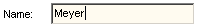
\includegraphics[width=0.4\textwidth]{./inf/SEKII/24_Java_GUI-Komponenten/JTextField.png}
\end{minipage}


Ein \myClass{JTextField} dient zur Darstellung und zur Eingabe von Text. Sowohl
der Anwender als auch das Programm können den dargestellten Text auslesen und
verändern.

Die Beschriftung vor einem \myClass{JTextField} gehört nicht zum Textfeld dazu,
sondern muss mit einem \myClass{JLabel} erzeugt werden:

\begin{lstlisting}
JLabel lblName = new JLabel("Name:");
panel.add(lblName);
\end{lstlisting}

Bei der Erzeugung des Textfeldes gibt man als Parameter die Anzahl der Zeichen
an, die im \myClass{JTextField} dargestellt werden sollen. Dadurch wird die
Länge der Komponente beeinflusst. Wenn der Benutzer mehr als die angegebenen
Zeichen eingibt, ist ein Teil des Textes nicht mehr sichtbar.

\begin{lstlisting}
JTextField tfName;
tfName = new JTextField(20);
panel.add(tfName);
\end{lstlisting}

Mit folgenden Methoden kann der Text der Komponente gelesen und verändert werden:

\begin{lstlisting}
public void setText(String t)
public String getText()
\end{lstlisting}

Mit

\begin{lstlisting}
public void setEditable(boolean b)
\end{lstlisting}

kann festgelegt werden, ob der Inhalt des Textfeldes durch den Anwender
editiert werden kann oder nicht.

\subsubsection{Ereignisbehandlung}

Es gibt zwei verschiedene Möglichkeiten, Ereignisse des Textfeldes zu
behandeln:

\begin{compactenum}[a)]
\item Wenn man sich nur dann benachrichtigen lassen möchte, wenn der Anwender
innerhalb des Textfeldes die ENTER-Taste drückt, implementiert man das Interface
\myClass{ActionListener}, das auch in Buttons verwendet wird. Mit folgender
Methode wird ein Objekt, das dieses Interface implementiert, bei einem
\myClass{JTextField} registriert:

\begin{lstlisting}
public void addActionListener(ActionListener l)
\end{lstlisting}

Die einzige Methode des Interfaces \myClass{ActionListener} sieht folgendermaßen
aus:

\begin{lstlisting}
public void actionPerformed(ActionEvent e)
\end{lstlisting}

\item Möchte man hingegen von jeder Änderung im Textfeld unterrichtet werden,
muss man einen \myClass{DocumentListener} auf das Modell des Textfeldes
registrieren:

\begin{lstlisting}
JTextField tfEingabe = new JTextField(20);
tfEingabe.getDocument().addDocumentListener(new DocumentListener() {
æ    /**
     *  insertUpdate() meldet, dass es eine Änderung gab
     */
æ    public void insertUpdate(DocumentEvent e) {}
æ    /**
     *  removeUpdate() meldet, dass ein Teil des Textes gelöscht wurde
     */
æ    public void removeUpdate(DocumentEvent e) {}
æ    /**
     *  changedUpdate() meldet, dass Attribute geändert wurde
     *  --> NICHT relevant für JTextField
     */
æ    public void changedUpdate(DocumentEvent e) {}
});
\end{lstlisting}
\end{compactenum}

\subsection{\myClass{JTextArea}}

Analog zu \myClass{JTextField} dient \myClass{JTextArea} zur Darstellung und zur
Eingabe von Text. Allerdings mehrzeilig. Es gibt mehrere Konstruktoren. Die
drei folgenden sind für uns besonders nützlich:

\begin{lstlisting}
public JTextArea()
public JTextArea(int rows, int columns)
public JTextArea(String t, int rows, int columns)
\end{lstlisting}

Man gibt im Konstruktor also die Größe (als Anzahl Zeilen und Anzahl Spalten),
sowie optional auch bereits den darzustellenden Text an. Beispiel:

\begin{lstlisting}
JTextArea taBrief;
taBrief = new JTextArea(20, 80);
panel.add(taBrief);
\end{lstlisting}

Der Konstruktor ohne Parameter erzeugt eine Komponente, die sich in den
aufnehmenden Container einpasst. Die wichtigsten Methoden sind wie schon bei
\myClass{JTextField}

\begin{lstlisting}
public void setText(String t)
public String getText()
\end{lstlisting}

Außerdem gibt es noch ein Methode, um Text an den bereits vorhanden Text
anzuhängen:

\begin{lstlisting}
public void append(String t)
\end{lstlisting}

\myClass{JTextArea} kümmert sich nicht darum einen zu breiten oder zu langen
Text über entsprechende Scrollbars erreichbar zu machen. Wer diese
Funktionalität braucht, muss die \myClass{JTextArea} in eine
\myClass{JScrollPane}-Komponente einbetten. Wie dies geht ist im Abschnitt zu
den komplexeren Komponenten im Zusammenhang mit \myClass{JList} erklärt.
